%!TEX program = xelatex
%!TEX TS-program = xelatex
%!TEX encoding = UTF-8 Unicode

% 学硕和专硕请将目录下对应的cls文件重命名为bjutthesis.cls
\documentclass[type=master]{bjutthesis}
\usepackage{bjutthesis}

% 定义所有的图片文件在 fig 子目录下
\graphicspath{{fig/}}

\begin{document}
\frontmatter
%封面与摘要中英文
\thusetup{
  udc={004}, %无需修改
  id={10005},%无需修改
  secretlevel={公开},%无需修改
  catalognumber={TP391.1}, %无需修改
  cstudent={S201761356},
  ctitle={基于多视角互补的SLAM算法研究},
  cauthor={谢帅},
  cdepartment={计算机技术},
  cmajor={计算机视觉},
  cdegree={工程硕士专业学位},
  csupervisor={马伟\ \ 副教授},
  ccollege={信息学部计算机学院},  
  cdate={2020年5月},
  corganization={北京工业大学},
  %
  %=========
  % 英文信息
  %=========
  etitle={Research on Multi-view Complementarity based SLAM},
  edegree={Master of Engineering},
  emajor={Computer Science and Technology},
  eauthor={Shuai Xie},
  esupervisor={Associate Professor Wei Ma}
}

% 定义中英文摘要和关键字
% 摘要中文大致一页长度 一段背景引入本文研究 说现有问题总结 本文贡献主要创新点 3个研究内容 3个创新点
\begin{cabstract}

中文摘要内容

\end{cabstract}

\ckeywords{同步定位与地图构建, 多视角互补, 捆绑优化, 线条优化, 复合特征优化}

\begin{eabstract}

English abstract

\end{eabstract}

\ekeywords{simultaneous localization and mapping, multi-view complementarity, bundle adjustment, line sequence optimization, complex feature optimization}

\makecover
% 目录
\tableofcontents
\bjutclearpage % 保证在偶数页结束本章节
%插图索引
\listoffigures
\bjutclearpage
% 表格索引
\listoftables
\bjutclearpage
% 公式索引
\listofequations
\bjutclearpage
% 符号表示 
% 写法一,单列列表,可以通过参数设置label宽度
% \begin{denotation} % [5cm]
%     \item[E] 误差
%     \item[T] 位姿
%     \item[$\bm{P}$] 三维点
% \end{denotation}  
% 写法二,两列表格,可以通过参数做单列或加三线等,参数格式同tabular
\begin{notation}%[p{1.4cm}<{\centering} p{5cm}<{\centering} p{1.4cm}<{\centering} p{5cm}<{\centering}]
    \hline
    符号 &含义 &
    符号 &含义\\
    \hline
    $\bm{P}$ &三维点 &        
    $\bm{L}$  &三维线\\
    $\bm{p}$ &二维点 &
    $\bm{l}$ &二维线\\
    $\bm{\pi}$ &平面 &
    $F$ &图像帧 \\
    $\bm{R}$ &旋转矩阵 &
    $\bm{t}$ &平移向量 \\
    $\bm{K}$  &相机内参矩阵 &       
    $\bm{T}$ &相机变换矩阵 \\
    $\bm{\mathcal{K}}$ & 直线投影的相机内参矩阵 &
    $\bm{\mathcal{H}}$ & 三维直线的相机变换矩阵 \\
    $\rho_h$ &Huber鲁棒代价函数 &       
    $\phi$ &投影函数\\
    $e$ &重投影误差 &
    $E$     &误差函数 \\
    $\bm{\Omega}$ &协方差矩阵 &
    $\Phi$ & 可信度 \\
    \hline
\end{notation}
\bjutclearpage
%%% 正文部分
\mainmatter
\chapter{章节标题}
\label{cha:introduction}

以下是简单的示例代码。

\section{二级标题}

\subsection{三级标题}

\subsubsection{四级标题}

\paragraph{段落标题}

这是一段文字。

\section{公式}
\label{sec:equation}

% 在不需要引用时,\label可以省略
\begin{equation}
\label{eq:error}
	E_p=\sum_i\rho_h(e_{p,i}^T\Omega_i^{-1}e_{p,i})
\end{equation}
其中,$\rho_h$为Huber鲁棒代价函数,增加了系统对于噪声点的鲁棒性……
% 方程组使用\left\{\begin{aligned}\end{aligned}\right.
% 矩阵考虑\begin{array}\end{array}

\subsection{引用}

上角标引用:ORB算法\cite{ORB},LSD算法\tcite{LSD},ORB-SLAM2\cite{ORB-SLAM2}算法。非角标引用:基于多视角互补的SLAM算法\mcite{xs2020SLAM}。

\subsection{插图}

\subsubsection{figure}

插入图片。多幅图像排列时,使用subfigure或minipage。
% 图片位置参数:! 不考虑美学, h 当前位置, t 页面顶部, b 页面底部, p 独立一页(一般不用)
\begin{figure}[htb]
	\centering
	% includegraphics支持width、height、scale参数
	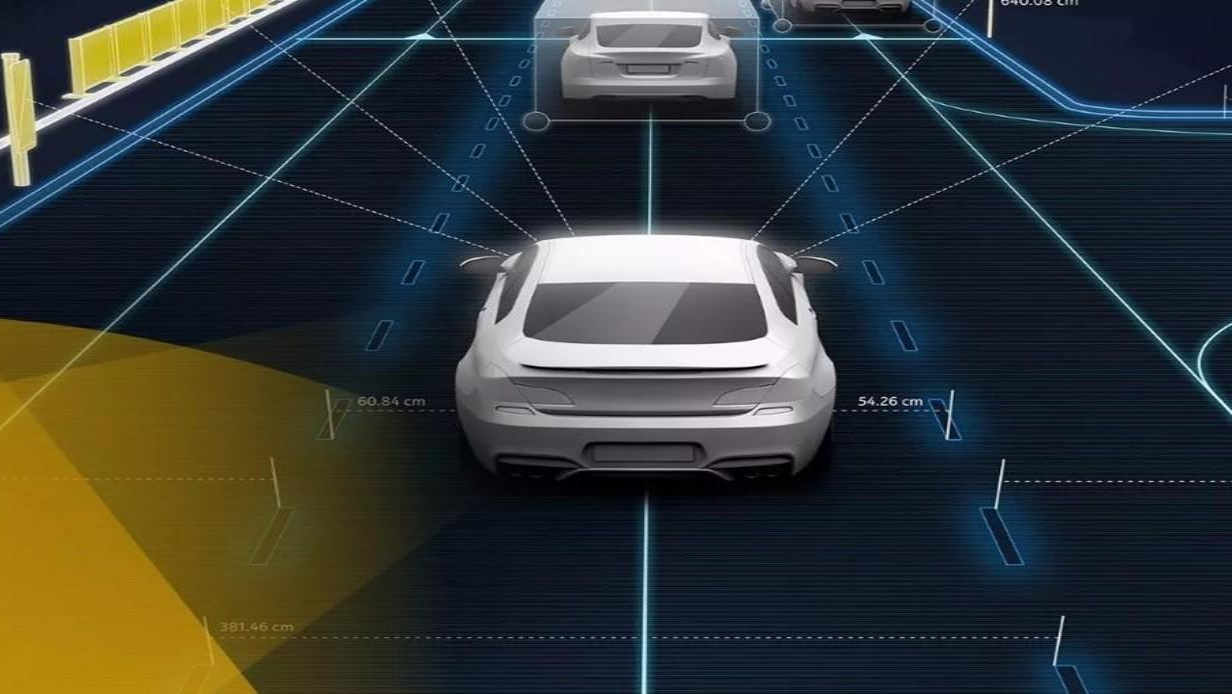
\includegraphics[width=0.7\textwidth]{autodrive.png}
	% footnotemark和footnotetext配合可以标注图片来源
	\caption{自动驾驶中的环境建模\protect\footnotemark[1]}
	\label{fig:introduction:autodrive}
	\addtocounter{figure}{-1}
	\renewcommand{\figurename}{Fig.}
	\caption{The environment reconstruction in automatic driving}
\end{figure}
\footnotetext[1]{图片来自于网络 http://auto.eastday.com/a/180720170248887.html}

\subsubsection{minipage}
minipage示例如图\ref{fig:line_optim:input}所示。

\begin{figure}[htb]
	\centering
	\begin{minipage}[t]{0.45\textwidth}
		\centering
		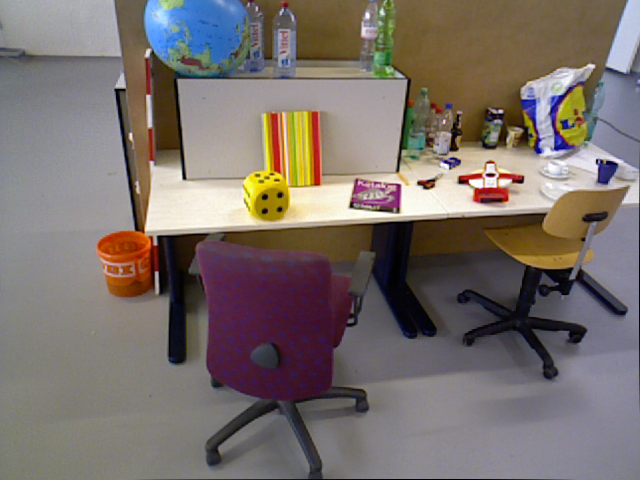
\includegraphics[width=0.8\textwidth]{tum-fr3-office-input1.png}
		\subcaption{场景输入图1}
		\label{fig:line_optim:input1}
	\end{minipage}
	\vspace{0.1in} %纵向间距,单位in或cm或pt等
	\begin{minipage}[t]{0.45\textwidth}
		\centering
		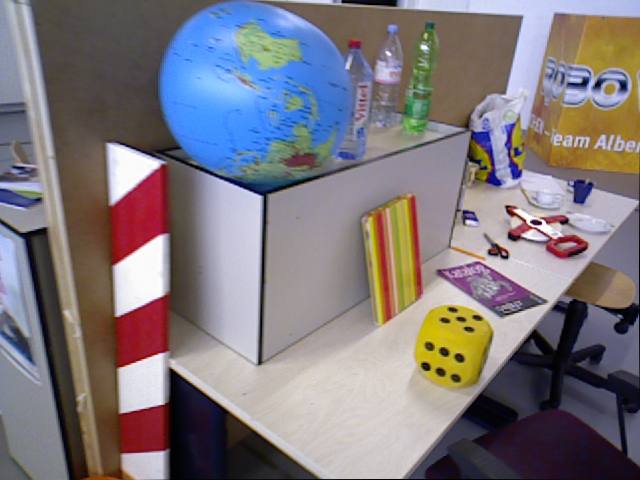
\includegraphics[width=0.8\textwidth]{tum-fr3-office-input2.png}
		\subcaption{场景输入图2}
		\label{fig:line_optim:input2}
	\end{minipage}
	\vspace{0.1in}
	\caption{TUM数据集{\itshape fr3\_long\_office}序列输入图}
	\label{fig:line_optim:input}
	\addtocounter{figure}{-1} %必须计数减一,否则上下中英标题的序号会递增
	\renewcommand{\figurename}{Fig.}
	\caption{The input images of {\itshape fr3\_long\_office} sequence in TUM dataset}
\end{figure}

\subsubsection{subfugure}
subfigure示例如图\ref{fig:line_optim:map}所示。

\begin{figure}[htb]
	\centering
	% subfigure[场景输入图像]{}
    \begin{subfigure}[b]{0.8\textwidth}
		\centering
		% 并排两个图像,也可以使用“\\”换行,改为纵向排列
        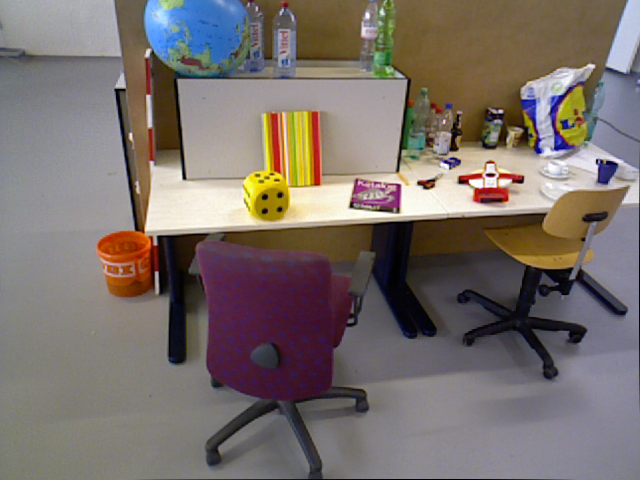
\includegraphics[width=0.45\textwidth]{tum-fr3-office-input1.png} %\\
        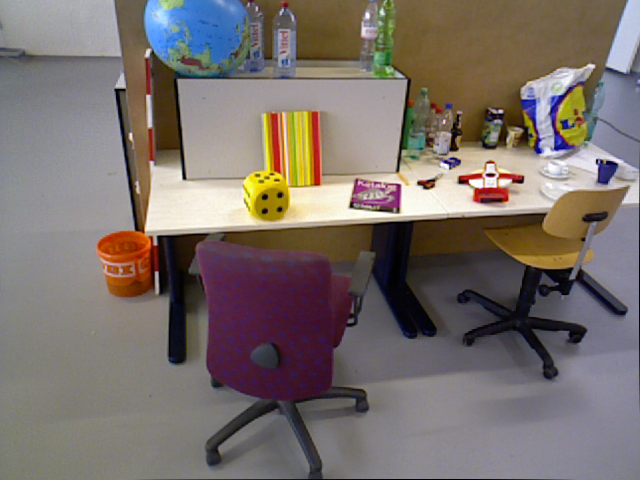
\includegraphics[width=0.45\textwidth]{tum-fr3-office-input1.png}
        \caption{场景输入图像}
    \end{subfigure}
    \vspace{0.3cm}
    \begin{subfigure}[b]{0.45\textwidth}
        \centering
        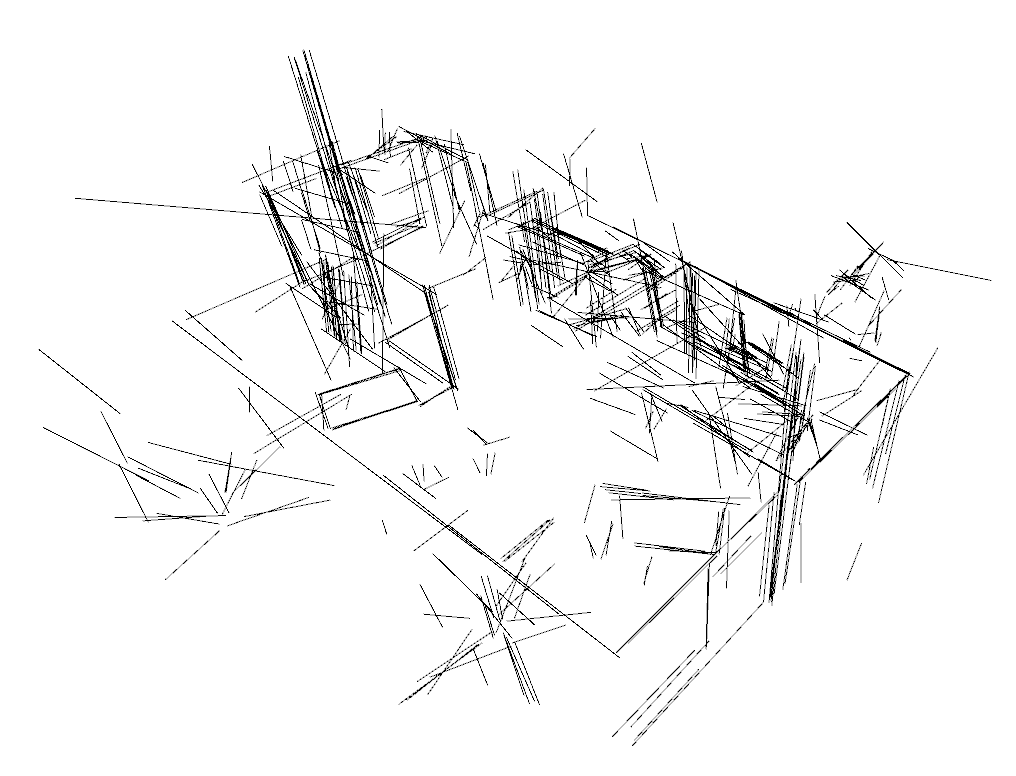
\includegraphics[width=0.9\textwidth]{line-map-TUM-fr3-office-lf.png}
        \caption{LF-SLAM算法的重建结果}
    \end{subfigure}
    \vspace{0.2cm}
    \begin{subfigure}[b]{0.45\textwidth}
        \centering
        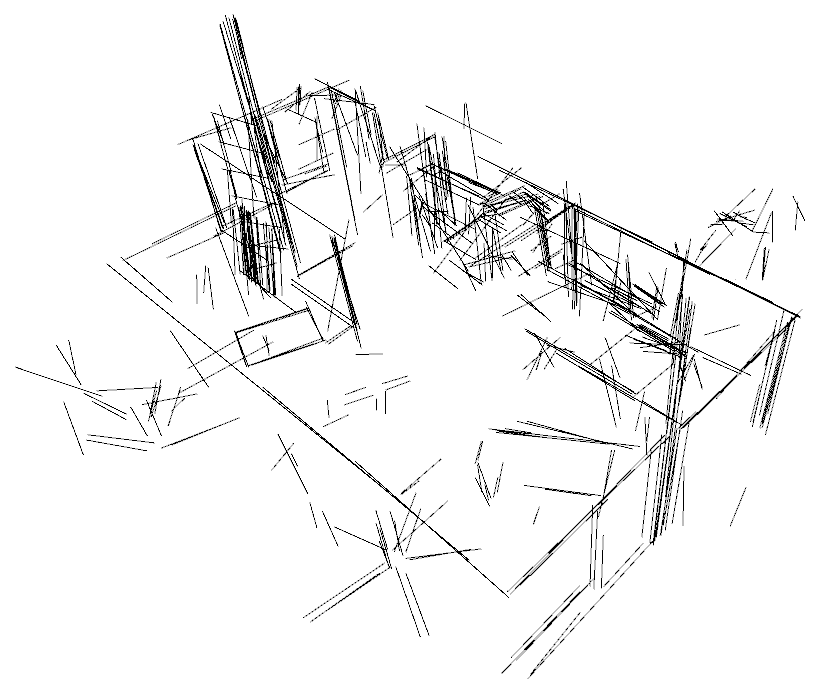
\includegraphics[width=0.9\textwidth]{line-map-TUM-fr3-office-ours.png}
        \caption{本章算法的重建结果}
    \end{subfigure}
    \vspace{0.2cm}
	\caption{在TUM {\itshape fr3\_long\_office}序列上的重建结果}
    \label{fig:line_optim:map}
    \addtocounter{figure}{-1}
    \renewcommand{\figurename}{Fig.}
    \caption{The results of mapping on {\itshape fr3\_long\_office} sequence in TUM}
\end{figure}

\subsection{表格}

表格示例如表\ref{table:running_time}所示。

\begin{table}[htb]
    \centering
    \small
    \caption{主流方法与本章方法的平均运行时间}
    \label{table:running_time}
    \addtocounter{table}{-1}
    \renewcommand{\tablename}{Table}
    \caption{The average running time of mainstream and the method in this chapter}
	\begin{center}
		% c 居中,l 左对齐,r 右对齐,t 指定列宽,顶部对齐,b 底部对齐,p 指定列宽,顶部对齐, m 指定列宽,居中对齐
		% | 表格竖线
        \begin{tabular}{c|p{2.2cm}<{\centering}|p{2.2cm}<{\centering}|p{2.2cm}<{\centering}|p{2.2cm}<{\centering}}
        \hline
		% 表头斜线,根据情况使用
		\diagbox[width=2.7cm,height=2cm,dir=NW]{数据集}{时间\\\ (ms)}{方法}	&ORB-SLAM	&PL-SLAM	&LF-SLAM &\ 本章方法\ 	\\
        \hline
        TUM			&20.6 		&45.9		&29.7	&26.8	\\
        7-Scenes	&20.0		&45.4		&28.6	&27.1	\\
		\hline
        \end{tabular}
    \end{center}
\end{table}

\subsection{列表}

\subsubsection{enumerate}
enumerate列表带编号,默认样式1.

\begin{enumerate}[1)]
	\item 分析现有SLAM框架的优势和不足,提出一种多视角互补的SLAM框架,该框架对现有框架做了改进,相比于现有框架,利用了观测数据的帧间约束信息,在位姿精度和重建效果方面提供了更大的提升空间。
	\item 在多视角互补框架下,结合多视角观测信息,提出一种可信度量方式,尽可能地降低不可靠特征对位姿优化带来的干扰,提升相机定位精度。
	\item 在多视角互补框架下,利用前后帧的观测信息,求解相机位姿和三维特征信息,同时也对局部帧的二维线条进行反向优化,提升线条完整度和端点的准确度,从而提升重建质量。
	\item 在多视角互补框架下,融合点线面特征,构建复合特征,在复合特征结构下,优化求解相机位姿和三维地图,提升优化速度和位姿精度,提高地图重建质量。
\end{enumerate}

\subsubsection{itemize}
itemize列表

\begin{itemize}
\item 第1章\quad 绪论

\item 第2章\quad 相关知识及数据集

\item 第3章\quad 基于多视角互补的SLAM框架

\item 第4章\quad 基于多视角互补的捆绑优化算法

\item 第5章\quad 基于多视角互补的线条优化算法

\item 第6章\quad 基于多视角互补的复合特征优化算法

\item 结论

\end{itemize}

\bjutclearpage
% \include{data/chap02}
% \include{data/chap03}
% \include{data/chap04}
% \include{data/chap05}
% \include{data/chap06}
% \include{data/chap07}
\begin{APP}


\end{APP}

\bjutclearpage
%\chapter{攻读硕士学位期间发表的学术论文}
%\label{cha:seven_achievements}
\begin{APP2}
\begin{enumerate}

    \item ……
    
\end{enumerate}
\end{APP2}

\bjutclearpage

\backmatter

%% 参考文献
\bibliographystyle{bjutthesis}
\bibliography{ref/refs}
\bjutclearpage

%% 致谢
% 如果使用声明扫描页,将可选参数指定为扫描后的 PDF 文件名,例如:
% \begin{acknowledgement}[scan-statement.pdf]
\begin{acknowledgement}

时光荏苒,三年的研究生生活即将结束……

% \mbox{}
% \begin{flushright}
%     \parbox[]{2.8cm}{谢帅}\\
%     \parbox[]{4.5cm}{二零二零年五月于北京}
% \end{flushright}

\bjutclearpage

\end{acknowledgement}


\end{document}
